\documentclass[12pt]{article}
\usepackage{parskip}
\usepackage[letterpaper, margin=1in]{geometry}
\usepackage{graphicx}
\usepackage{amsmath}
\usepackage{pdflscape}
\usepackage{tikz}
\usepackage{fancyhdr}
\renewcommand{\headrulewidth}{0pt}
\usepackage{titlesec}
\fancypagestyle{lscapedplain}{%
  \fancyhf{}
  \fancyfoot{%
    \tikz[remember picture,overlay]
      \node[outer sep=1cm,above,rotate=90] at (current page.east) {\thepage};}
}
\graphicspath{{./images/}}
\title{ELECENG 2EI5 Project 3}
\author{Raeed Hassan \\ hassam41 \\  \\ McMaster University}
\begin{document}
\maketitle
\pagebreak

\begin{enumerate}
\item Hand design
\begin{enumerate}
    \item
    The circuit topology chosen was the common collector amplifier. The specifications of the problem generally do not favour any amplifier circuit topology over another, therefore the common collector was chosen simply because it would make the task of observing linearity between the input and the output easier due to there being close to no voltage gain ($\frac{v_o}{v_{in}} \approx 1$). 
    \item
    The specific device chosen is the NPN simply because BJTs are more commonly used than MOSFETs in discrete amplifiers. None of the advantages of using MOSFETs in amplifier circuits (cheaper fabrication costs and better performance with active loads) apply in this scenario, therefore there was no reason to use one. 
    \item
    To determine the values of the components used, we first need to determine what components are necessary to meet the specifications. First, an amplifier circuit was simulated with no additional components other than the BJT, and the two specified resistors. We can observe the behaviour of the circuit to determine if any additional components are required or any modifications need to be made.   
    \item
    The circuit simulated with no additional components meet all the specifications, therefore no additional calculations were performed to determine component values. The only specifications of the circuit that needed to be tweaked were the DC bias of the input, and the voltage entering the collector, and these values were found through trial and error in simulation. The only calculation needed was to determine the attenuation. To calculate the attenuation, we determined the input resistance of the amplifier circuit (calculated in simulation), which ranged from $42k\Omega$ to $58k\Omega$. The attenuation was calculated less than 10\% for this entire range as the value of $\frac{R_{in}}{R_s + R_{in}}$ ranged from $0.997$ to $0.998$.
    \item
    All specifications that can be calculated in the hand design were met. The final design can be seen in Figure \ref{fig:Schematic}. The source has an internal resistance of $100\Omega$, the load has an input resistance of $100\Omega$, and the attentuation is less than 10\%. The linearity of the circuit is determined in simulations and measurements.
\end{enumerate}
\item Simulations
\begin{enumerate}
    \item 
    A transient analysis with stop time of 10ms was conducted, and the output voltage (voltage drop across $R_L$) and input voltage (voltage from function generator producing sine voltage of amplitude $0.5V$) were plotted. The results can be seen in Figure \ref{fig:Simulation}.
    \item 
    The SPICE model for the NPN that is used is the model provided by the manufacturer of the NPN (Onsemi 2N3904) used in the circuit built in the experimental portion of the lab.
    \item 
    The simulations matched the expected behaviour based on the hand design. The AC voltage gain was approximately 1, with no phase shift. There was good linearity and no visible attenuation, and all other specifications of the problem were met. 
\end{enumerate}
\item Measurement
\begin{enumerate}
    \item 
    The only measurements performed on the circuit were measuring the input and output voltages of the circuit. The input voltage was measured by connecting the positive terminal of scope 2 to the output of wavegen 1, and connecting the negative terminal of scope 2 to ground. The output voltage was measured by connecting the positive terminal of scope 1 to the emitter of the NPN, and connecting the negative terminal of scope 1 to ground.
    \item 
    All specifications of the design problem were met. The source that is connected to the amplifier circuit is connected a $100\Omega$ resistor. The amplifier circuit is connected to a $100\Omega$ load resistor. There is no notable attentuation present in the input or output voltages. There is good linearity between the input and output voltages. 
    \item 
    There are no discrepanies between the measurements with the simulations or the hand design.
    \item 
    All specifications of the design problem were met.
\end{enumerate}
\end{enumerate}

\pagebreak
\begin{landscape}
  \pagestyle{lscapedplain}
  \appendix
  \section{Figures}
  \begin{figure}[ht!]
    \begin{minipage}[b]{0.5\linewidth}
        \centering
        \includegraphics[width=0.9\linewidth]{images/Schematic.png} 
        \caption{Schematic}
        \label{fig:Schematic}
        \vspace{4ex}
    \end{minipage}%%
    ~
    \begin{minipage}[b]{0.5\linewidth}
        \centering
        \includegraphics[width=\linewidth]{images/Simulation.png} 
        \caption{Simulation of input (cyan) and output (green) voltages}
        \label{fig:Simulation}
        \vspace{4ex}
    \end{minipage}
    \begin{minipage}[b]{0.5\linewidth}
        \centering
        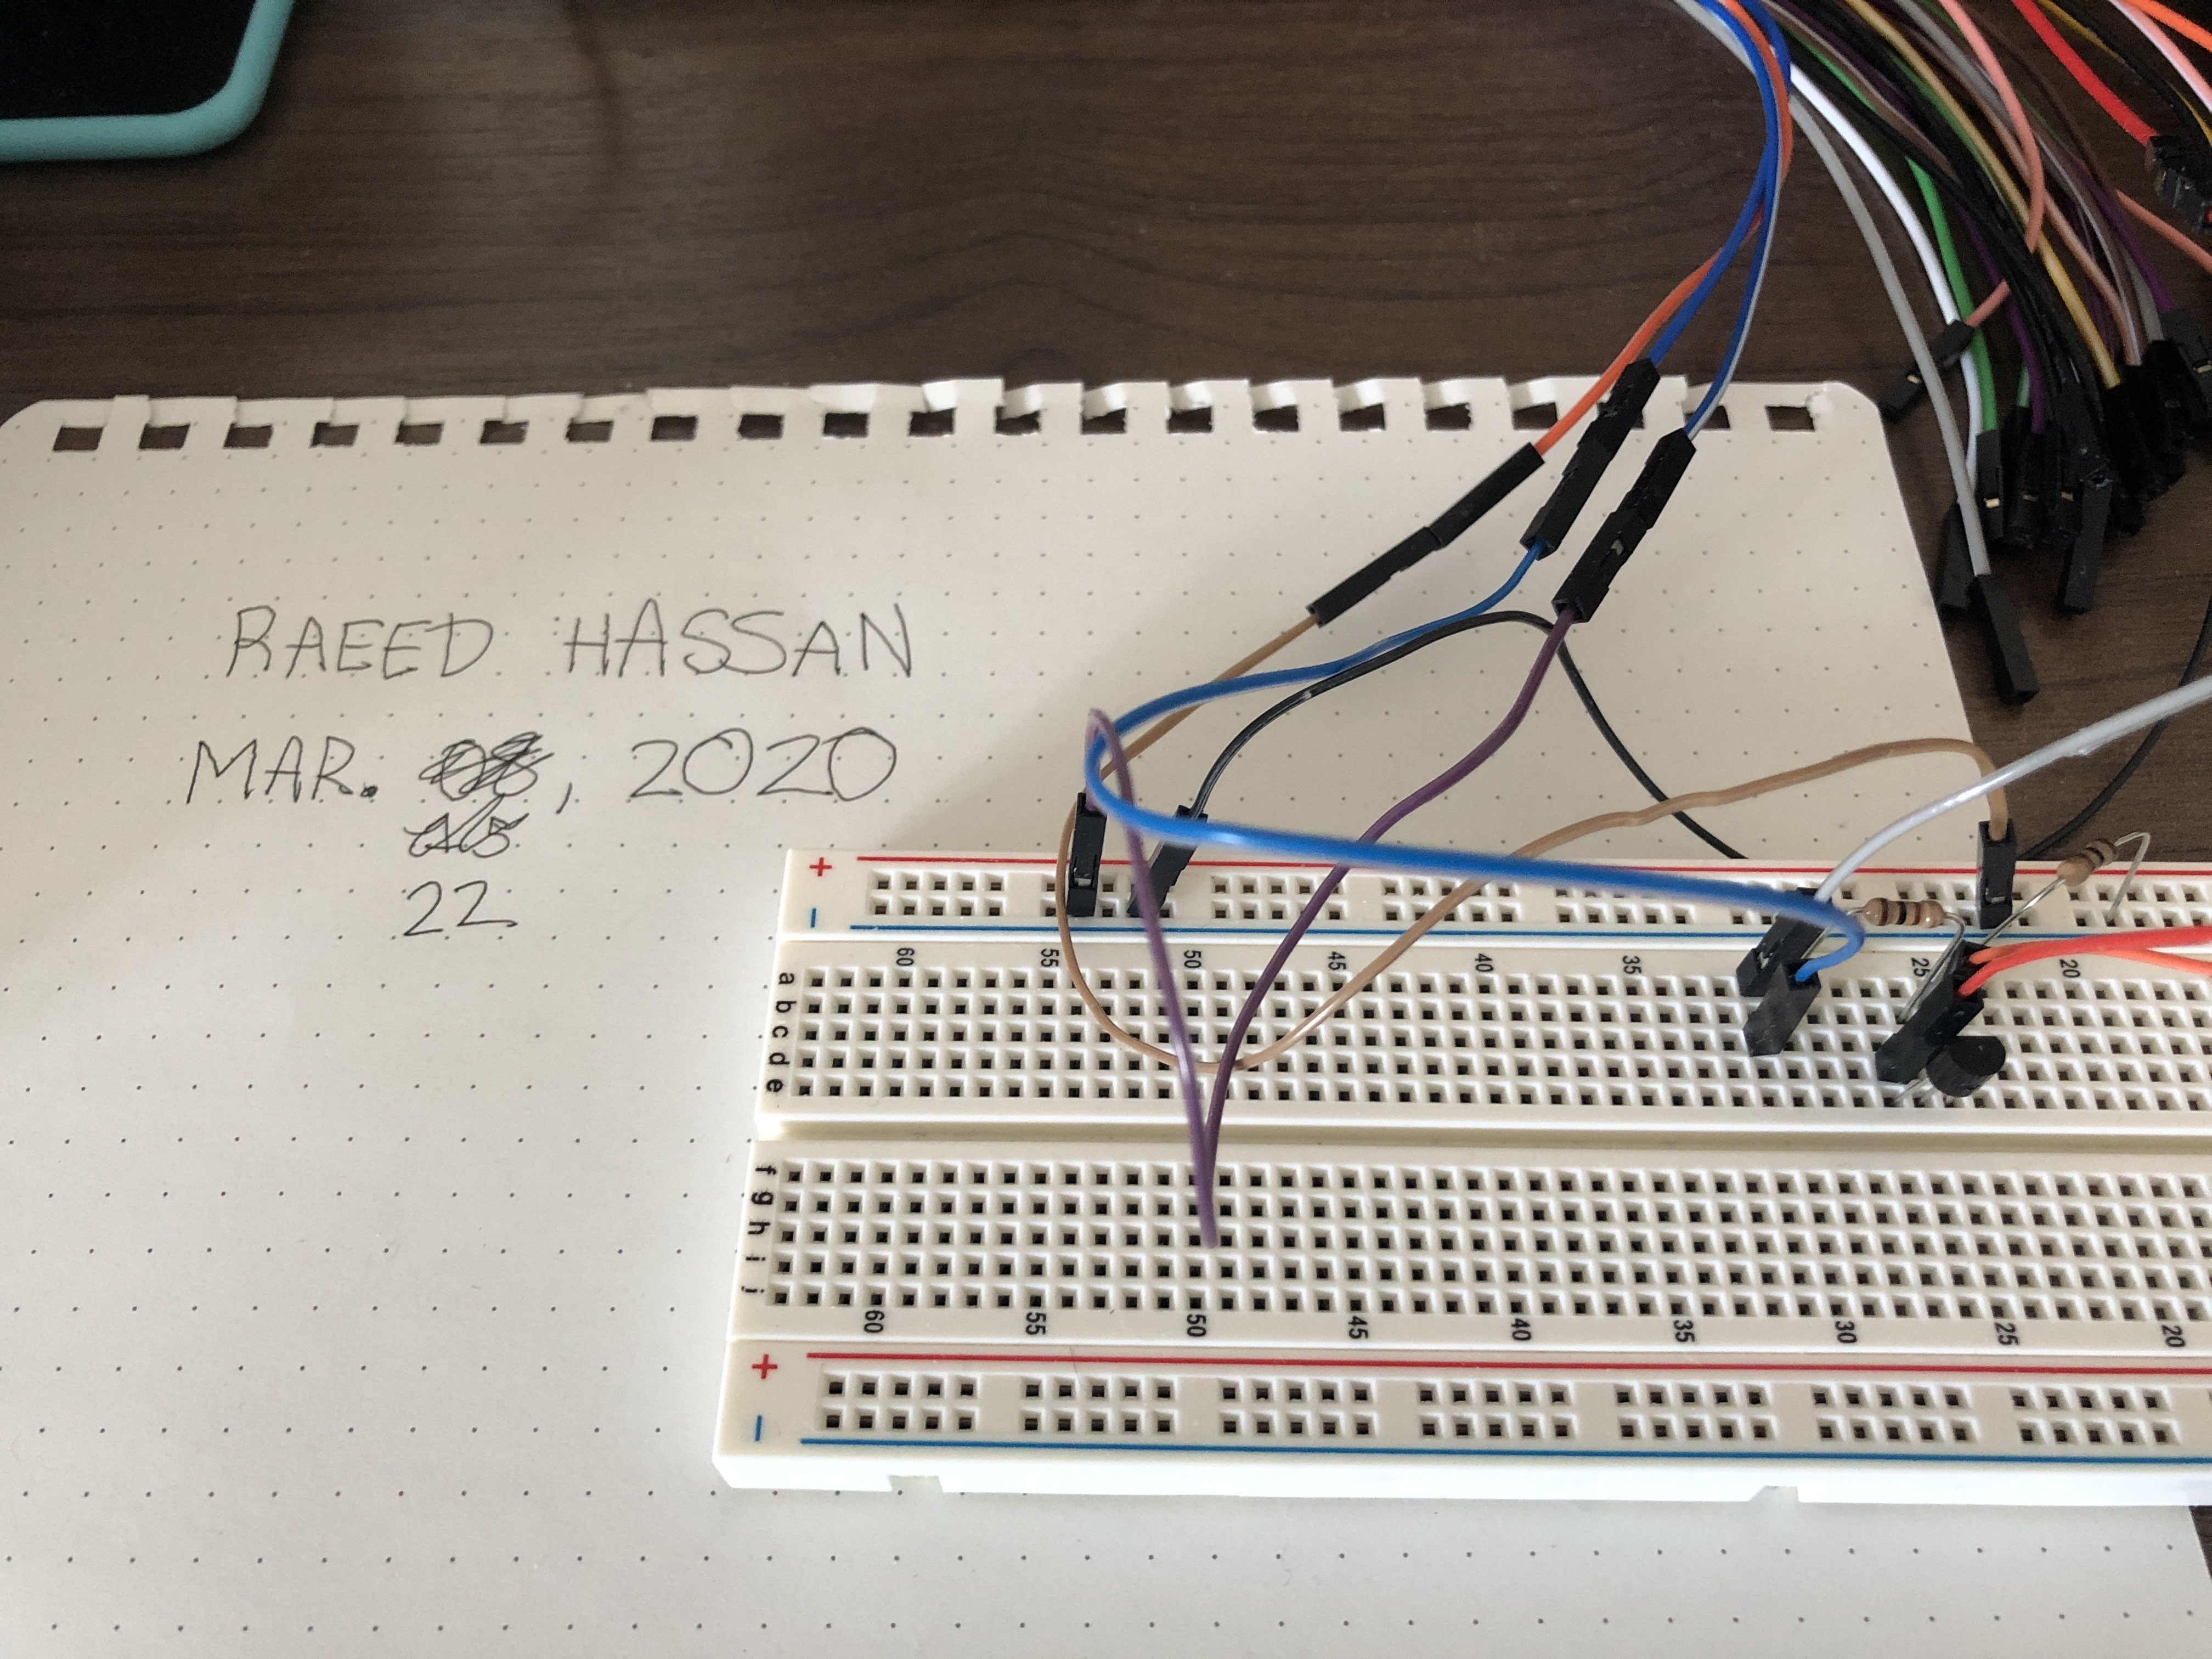
\includegraphics[width=0.7\linewidth]{images/Circuit.png} 
        \caption{Physical circuit} 
    \end{minipage}%%
    \begin{minipage}[b]{0.5\linewidth}
        \centering
        \includegraphics[width=\linewidth]{images/Measurements.png} 
        \caption{Measurements of input (blue) and output (yellow) voltages} 
    \end{minipage}%%
\end{figure}
\end{landscape}
\end{document}